\chapter{Fundamentals and background}
\label{cha:Fundamentals}

This chapter gives details of the various components used in implementation
of the system described by this thesis. This will include the Software
tools and techniques used to program the target design as well as the Hardware
components essential to achieve the proposed topologies for the FPGAs. The chapter
also introduces the base system and its background which is extended in the thesis.

\section{Hardware and Software Platform}

This section describes the hardware and the software platform used in the
thesis for implementing and evaluating the extended design. The first subsection
gives an overview of BittWare 520N board followed by and description of software
setup using Intel FPGA SDK for OpenCL used to implement the FPGA kernels.

\subsection{BittWare 520N}

The BittWare 520N FPGA acceleration boards are used for the development
and evaluation of the proposed system. The BittWare's p520\_max\_sg280l BSP
provided with the board is used along with the board which provided support for
\begin{enumerate}
    \item Intel Stratix 10 FPGA GX2800 capable for providing up to 10 TFLOPS of single
    precision floating point performance
    \item DDR4 SDRAM memory divided into 4 banks with 8GB each giving a total memory of 32GB with
    a transfer rate of 2400 MT/s
    \item Four 100/40/25/10G QSFP28 Network Ports supported in the
    BSP as 4x40G Intel OpenCL external I/O channels
    \item 16-lane PCI-Express Gen 3.0 for high speed host to FPGA data transfers (The current version of
    the BSP supports only 8 PCIe 3.0 lanes)
\end{enumerate}

The Intel Stratix 10 FPGA GX2800 FPGA belongs to the current generation of the high-performance FPGA
family with new Intel Hyperflex™ core architecture which gives higher bandwidth and processing
performance to the FPGAs. The resource summary for the FPGA is given in table \ref{tab:res_sum}
which shows the high computation capabilities of the FPGAs
\begin{table}[]
    \centering
    \caption{Intel Stratix 10 FPGA GX2800 Resource summary}
    \label{tab:res_sum}
    \begin{tabular}{lr}
    \hline
    \textbf{Resources} & \multicolumn{1}{c}{\textbf{\#}} \\ \hline
    Logic elements (LEs) & 2,753,000 \\ \hline
    Adaptive logic modules (ALMs) & 933,120 \\ \hline
    M20K memory blocks & 11721.00 \\ \hline
    M20K memory (Mb) & 229 \\ \hline
    MLAB memory (Mb) & 15 \\ \hline
    DSP & 5,760 \\ \hline
    \end{tabular}%
\end{table}

\subsubsection*{QSFP Network Ports}

The BittWare boards also contains 4 QSFP Network Ports which
are connected to the FPGA transceivers to provide high speed network communication. As mentioned
previously these ports are used in this thesis to setup FPGA-to-FPGA networks to transfers data
and reduce communication latency. The connections between the FPGAs are done using
high speed fiber optic transceivers and cables capable of high speed long and short distance communications.
The current version of the BittWare BSP supports 40 Gbits/s speed which is used for all calculation in this thesis.

\subsection{Intel FPGA SDK for OpenCL™}

Intel FPGA SDK for OpenCL™ v18.0.1 Pro and v18.1.1 Pro is used for the development,
debugging and synthesizing of the OpenCL kernels developed in this thesis.
Intel MPI Library v18.0.3 is used for the MPI communication between the nodes
for distributed setups. ParMETIS v4.0.3 is used for implementation of the partitioning
scheme in the MIDG2 application.

The software development is based on the existing MIDG2 MPI FPGA code base
which is described in section \ref{sec:midg2_base}. The software package consists
the \texttt{host application} which implements the mesh handling, partitioning,
coefficient initialization and OpenCL™ platform initialization and control
logic. The package also contains the OpenCL™ kernels which implement
the computation logic of the DG method for distributed FPGA system using
MPI+PCIe for communication between the FPGAs. This design is used as the base
for the thesis and is extended in the thesis to include IO channels for communication
in different topologies.

\subsubsection{OpenCL application development}

The OpenCL framework provides a programming environment for implementing
applications for heterogenous systems which can include CPUs, GPUs,
DSPs and FPGAs. An OpenCL™ application is divided into two parts \texttt{Host application} and
\texttt{OpenCL KERNEL}. The \texttt{Host application} is executed on the \texttt{HOST} PC,
mostly the CPU and the \texttt{OpenCL KERNEL} is executed on a separate hardware accelerator
such as a GPU or FPGA. The \texttt{Host Application} can be implemented using
C or C++ programming language and use the OpenCL runtime APIs to configure, control
and execute programs on the target platform device. A \texttt{OpenCL KERNEL} is
implemented using the OpenCL kernel programming language which is based on C/C++
and includes special programming constructs and keywords to use additional features
for a target platform. The \texttt{OpenCL KERNEL} implements the computational
logic which can be offloaded to the additional accelerator to speedup the computation.

For Intel FPGAs the \texttt{Host application} and \texttt{OpenCL KERNEL} are compiled separately.
The \texttt{OpenCL KERNEL} code for FPGA is synthesized into binary using the Intel FPGA SDK for OpenCL
offline compiler. \texttt{Host application} is compiled with the OpenCL runtime library and uses the
OpenCL application runtime provided by the Intel to configure and execute the synthesized binary on the FPGA device.


% \subsubsection{Loop Pipelining and unrolling }
% \TODO{Add section to describe loop pipeline in nexted loops}
% \TODO{Add section to describe Memory banking and benfits in OpenCL™ kernels}

\subsection{OpenCL™ Serial IO channels}

The communication over the QSFP ports can be implemented using OpenCL™ by using the
Intel's OpenCL™ IO channels support. The IO channels can be used to stream data
directly between kernels and I/O using explicitly named channels. The declaration
of these channels should be included in the \texttt{board\_spec.xml} using the
\texttt{channels} element. The BittWare BSP \texttt{p520\_max\_sg280l} provides
4 Tx and 4 Rx IO channels for the 520N board as shown in the listing \ref{code:board_spec}
which interface to the 4 QSFP ports on the board.
In order to use these I/O channels in the OpenCL kernel,
an \texttt{io} attribute is included in the channel declaration along with id of
the interface which is specified in the \texttt{board\_spec.xml}.

\begin{XmlCode}[caption=IO channels desciption in \texttt{board\_spec.xml}, frame=tlrb, label=code:board_spec]
<channels>
    <interface name="board" port="io_to_dev_ch0" type="streamsource" width="256" chan_id="kernel_input_ch0"/>
    <interface name="board" port="dev_to_io_ch0" type="streamsink" width="256" chan_id="kernel_output_ch0"/>
    <interface name="board" port="io_to_dev_ch1" type="streamsource" width="256" chan_id="kernel_input_ch1"/>
    <interface name="board" port="dev_to_io_ch1" type="streamsink" width="256" chan_id="kernel_output_ch1"/>
    <interface name="board" port="io_to_dev_ch2" type="streamsource" width="256" chan_id="kernel_input_ch2"/>
    <interface name="board" port="dev_to_io_ch2" type="streamsink" width="256" chan_id="kernel_output_ch2"/>
    <interface name="board" port="io_to_dev_ch3" type="streamsource" width="256" chan_id="kernel_input_ch3"/>
    <interface name="board" port="dev_to_io_ch3" type="streamsink" width="256" chan_id="kernel_output_ch3"/>
</channels>
\end{XmlCode}

A example kernel code is shown in the listing \ref{code:board_spec} where two OpenCL
kernels \texttt{sender} and \texttt{collector}
are implemented to use the IO channels. The kernels use one TX (\texttt{ch\_eth\_in})
and one RX (\texttt{ch\_eth\_out}) channel to
communicate in the \texttt{sender} and \texttt{collector} kernels.
\texttt{ch\_eth\_in} and \texttt{ch\_eth\_out} are declared with \texttt{io} attribute
to interface with the external channels \texttt{kernel\_input\_ch0} and \texttt{kernel\_output\_ch0} respectively.
The channels should be declared with a datatype (\texttt{float8} in this case)
suitable to hold the 256 bits wide data which is the current width of the channels.
After the declaration, the channels can be used by the kernel similar to standard OpenCL™
channels using \texttt{write\_channel\_intel} and \texttt{read\_channel\_intel} APIs to write
to the TX channel and read from the RX channel as shown.

\begin{CppCode}[caption=IO channels usage example in a OpenCL™ kernel, frame=tlrb, label=code:board_spec]
#pragma OPENCL EXTENSION cl_intel_channels : enable

channel float8 ch_eth_in __attribute((io("kernel_input_ch0")));
channel float8 ch_eth_out __attribute((io("kernel_output_ch0")));

__kernel void __attribute__ ((max_global_work_dim(0)))
sender(int length, __global float8 * restrict input)
{
    for(int i=0; i<length; ++i)
        write_channel_intel(ch_eth_out, input[i]);
}

__kernel void __attribute__ ((max_global_work_dim(0)))
collector(int length, __global float8 * restrict output)
{
    for(int i=0; i<length; ++i)
        output[i] = read_channel_intel(ch_eth_in);
}
\end{CppCode}

\section{Nodal Discontinuous Galerkin Method}
\label{sec:dgtd}

The \ac{DGTD} \cite{hesthaven_nodal_2008} is used to find solutions
for partial differential equations (PDE) numerically. This method is efficient in
producing results with computers as it relies on mathematical calculations on elemental basis.
This allows to perform computation in parallel on similar or different hardware helping to
solve problems from different domains quickly. \ac{DGTD} method is particularly popular for applications
in the domains such as fluid mechanics, plasma physics and electrodynamics.

\subsection{DGTD to solve Maxwell equations}
\label{sec:dgtd_maxwell}

\textcite{Hesthaven_190449} presented the use of \ac{DGTD} to solve time-domain Maxwell's equations with
an 1D and 2D examples and the extension to 3D is explained in \cite{hesthaven_nodal_2008}. This section
briefly describes the formulations and steps involved for getting the solutions which are
used as the basis for implementation in the application used in this thesis to simulate
electromagnetic flux values for a given material.

The basic equation involved in computation of the electromagnetic flux is Maxwell's equations. The
three dimensional time-dependent Maxwell's equations \cite{hesthaven_nodal_2008} is written as:
\begin{equation}\label{eqn:maxwellbase}
    \mu \frac{\partial{\textbf{H}}}{\partial{t}} = - \nabla \times \textbf{E},\varepsilon \frac{\partial{\textbf{E}}}{ \partial{t}} = - \nabla  \times \textbf{H}
\end{equation}
the conservation form of the equation can be expressed as:
\begin{equation}\label{eqn:maxwell}
    \mathcal{Q}\frac{\partial\textbf{q}}{\partial{t}}  + \nabla  \cdot \mathcal{F} = 0
\end{equation}
where
\begin{equation}\label{eqn:maxwellexpansion}
\textbf{q} =  \begin{bmatrix}\textbf{H} \\ \textbf{E} \end{bmatrix},
\mathcal{Q} =  \begin{bmatrix} \mu & 0 \\ 0 &  \varepsilon \end{bmatrix},
\mathcal{F} = \begin{bmatrix}  - \widehat{n} \times \textbf{E} \\ \widehat{n} \times \textbf{H} \end{bmatrix} = \begin{bmatrix} \textbf{F}_H \\ \textbf{F}_E \end{bmatrix}
\end{equation}

\textbf{H} and \textbf{E} are the magnetic and electric vector fields in
three dimensions which are function of the positional coordinates and time
$ (\tilde{x},\tilde{y}, \tilde{z}, \tilde{t}) $, $ \mathcal{Q} $ defines the magnetic permeability
$ \mu(x) $ and the electric permittivity $ \varepsilon(x) $ of the material.

Now considering that we have an object composed of a single type of material with known $ \mathcal{Q} $
values, the DG method can be used to solve the equation \ref{eqn:maxwell} by discretization of the
computation domain $ \Omega $ (whole of the object) spatially. In 3D, this can be achieved by dividing the object
into K tetrahedral elements and computing the local approximated solution $ u_h^k(x,t) $ for
each element $ D^k \in K $. This local solution is computed for a defined polynomial order $ N $ such that,
$ h \in N $ represents the $ h^{th} $ polynomial of $ D^k $ and is called the nodal point.
Now for a given polynomial order $ N $, the local solution can be expressed \cite{hesthaven_nodal_2008} as:
\begin{equation}\label{eqn:nodal_form}
    x \in D^k \ : \ u^k_{h}(\textbf{x}, t) \; = \; \sum_{n=1}^{N_p} \hat{u}_n(t) \psi_{n}(\textbf{x}) \; = \; \sum_{i=1}^{N_p} u^k_{h}(\textbf{x}_{i}, t) l^k_{i}(\textbf{x})
\end{equation}
where $ l^k_{i}(\textbf{x}) $ is the multidimensional Lagrange polynomial and $ \psi_{n}(\textbf{x}) $
is a three-dimensional polynomial basis.

In equation \ref{eqn:nodal_form}, the $ N_p $ denotes the number of nodal points per element $ D^k $
and depends on the polynomial order $ N $ which is given by:
\begin{equation}\label{eqn:nprelation}
    N_p = \frac{(N+1)(N+2)(N+3)}{6}
\end{equation}

Now that we know the basis for computation of local approximated solutions for elements,
the local solutions can be combined to give an approximation of the global solution. This is
done by using an operator to combine the local solutions $ u_h^k(x,t) $ elementwise
except for nodal points on the faces. The nodal points
on the faces of the tetrahedra are part of two adjacent $ D^k $ elements and have two different
field values require coupling of the local solution. The coupling of the solution is done
by computing the electric and magnetic field differences \cite{kenter_opencl-based_2018} $\Delta \textbf{E}
= \textbf{E}^+-\textbf{E}^-, \Delta \textbf{H} = \textbf{H}^+ - \textbf{H}^-$.
The global approximate solutions is then achieved from the local solutions \cite{kenter_opencl-based_2018, busch_discontinuous_2011}
by a pair of \ac{ODE} for the semi-discrete system derivation which combines the local and global
field values as explained in \cite{hesthaven_nodal_2008}:
\begin{equation}\label{eqn:pde_e}
\epsilon^k \frac{\partial \textbf{E}^k}{\partial t} = \textbf{D}^k \times \textbf{H}^k
+ (\mathcal{M}^k)^{-1}\mathcal{F}^k \left( \frac{\Delta\textbf{E}-\hat{n} \cdot (\hat{n} \cdot \Delta \textbf{E})+Z^+ \hat{n} \times \Delta \textbf{H} }{\overline{Z}} \right)
\end{equation}
\begin{equation}\label{eqn:pde_h}
    \mu^k \frac{\partial \textbf{H}^k}{\partial t} = - \textbf{D}^k \times \textbf{E}^k
    + (\mathcal{M}^k)^{-1} \mathcal{F}^k \left ( \frac{\Delta \textbf{H} -\hat{n} \cdot (\hat{n} \cdot \Delta \textbf{H})-Y^+ \hat{n} \times \Delta \textbf{E}}{\overline{Y}} \right)
\end{equation}
The $ (\mathcal{M}^k) $ is mass matrix, $\mathcal{F}^k$ is face matrix, $\hat{n}$ outwardly
pointing normal vector to the element face where the flux is calculated. The $ Z^\pm $ and $Y^\pm$ is the impedance and the conductance of the material.

The solution of these \ac{ODE}s require time discretization. The Runge-Kutta
scheme introduced in \cite{shu_total-variation-diminishing_1988} is used
\cite{hesthaven_nodal_2008, kenter_opencl-based_2018} to integrate the
equations in time. The timesteps are chosen in way such that they are small
and ensure that the timestep error can be neglected. In the implementation used
in this thesis, the timestep is computed by calculating the smallest distance between two nodal points.

\section{\acf{MIDG2}}
\label{sec:midg2_base}

\ac{MIDG2} is a open source C/C++ based application which implements the \ac{DGTD} method for solving
Maxwell's equations for 1D, 2D and 3D. It uses K non-overlapping tetrahedra elements as described in
section \ref{sec:dgtd_maxwell} for computing the flux values for a given object. This section
will give an overview of the application implementation along with improvements done to use
multiple FPGAs to offload the computation and speed up the execution time.

The original MIDG2 implementation supports parallelization using \ac{MPI} for multiple CPUs and
uses OCCA \footnote{\url{https://libocca.org}} to provide support for acceleration with GPU
using CUDA and OpenCL™. The object for which the flux is to be computed is represented as
an unstructured mesh of K non-overlapping tetrahedral elements as shown in fig \ref{fig:mesh}.
This mesh is generated using the tool Tetgen\footnote{\url{http://wias-berlin.de/software/tetgen/}}
which is an open source tool to generate meshes. The tetrahedra within the mesh are
identified with their vertices. The application uses three vectors VX, VY and VZ
to store the coordinates of each of the vertices. The application performs the steps
which are formulated in section \ref{sec:dgtd_maxwell} using mesh and additional
inputs which include mass matrixes and Runge-kutta time step constants to compute the
flux values for a given polynomial order.
\begin{figure}[h]%
    \centering
    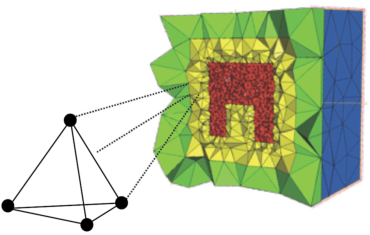
\includegraphics[width=0.6\textwidth]{images/mesh}
    \caption{K element mesh with tetrahedra elements for split-ring resonator object taken from \cite{forstner_discontinuous_nodate}}
    \label{fig:mesh}
\end{figure}

The parallelization of computation can be achieved in this implementation by dividing
the mesh into partitions. As the \ac{DGTD} algorithm works by first computing individual
local solution for the elements and use an approximation operator to combine the local
solutions element wise all $Ks$,
a partitioning scheme which uses surfaces as boundaries can be performed such that,
computation of each individual partition is performed by a separate
process/thread/core/system and the shared surface data is shared at each time step
between them using a communication infrastructure. The partitioning in MIDG2 is
achieved using an open source tool ParMETIS\footnote{\url{http://glaros.dtc.umn.edu/gkhome/metis/parmetis/overview}},
which is effective in partitioning meshes for a distributed system for equal load sharing.
The MIDG2 uses \ac{MPI} for implementing a distribution and communication scheme which
allows to use multiple nodes/MPI ranks speedup the computation by distributing the computation load.
The step wise process for partitioning and distribution is shown in fig \ref{fig:partitioning}.
\begin{figure}[h]%
    \centering
    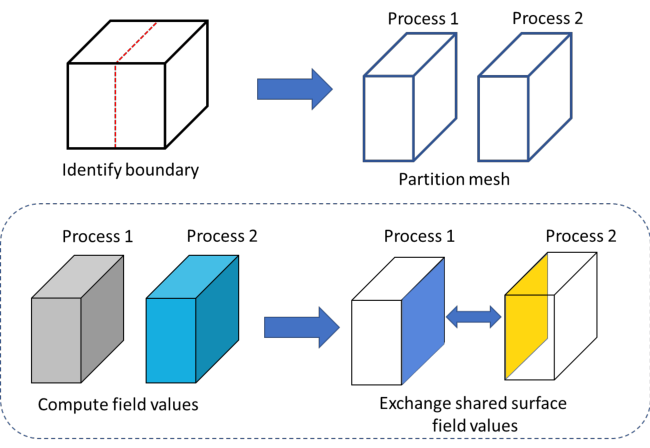
\includegraphics[width=0.7\textwidth]{images/partition_proc}
    \caption{Parallelization achieved with partitioning and processing by multiple processes}
    \label{fig:partitioning}
\end{figure}

\section{FPGA implementation for DGTD (MIDG2 FPGA)}
\label{sec:fpga_dg}

\textcite{kenter_opencl-based_2018} extended the original MIDG2 implementation to use
FPGAs to accelerate the computation for a single FPGA system. This implementation
uses Intel™ FPGA SDK for OpenCL™ to implement three compute kernels viz. \texttt{VOLUME} kernel,
\texttt{SURFACE} kernel and \texttt{RK} kernel which perform the computation steps for the \ac{DG} solver.
The kernels developed were optimized to utilize the capabilities of the FPGA such
as parallelization of operations by replication, optimizing memory access by using
local memory for storing constant data, using multiple memory access channels to allow parallel data
reads/writes for higher bandwidth with lower stalls.
The structure of the OpenCL™ kernels for this implementation is shown in figure  \ref{fig:singlefpga_kernstruc}
which shows pipeline structure developed for acceleration with the single FPGA.
The IO kernels for \texttt{SURFACE} and \texttt{VOLUME} act as memory interface kernels which
access the global memory as source and sink for data. Use for multiple
kernels in such way along with the Intel™ FPGA OpenCL™
channels, create a pipeline structure for the \texttt{VOLUME} and surface compute kernels
which allows to start computation on a nodal point in each cycle.

The complete implementation details along with performance evaluation for the design
is described in \cite{kenter_opencl-based_2018}.

\begin{figure}[ht]%
    \centering
    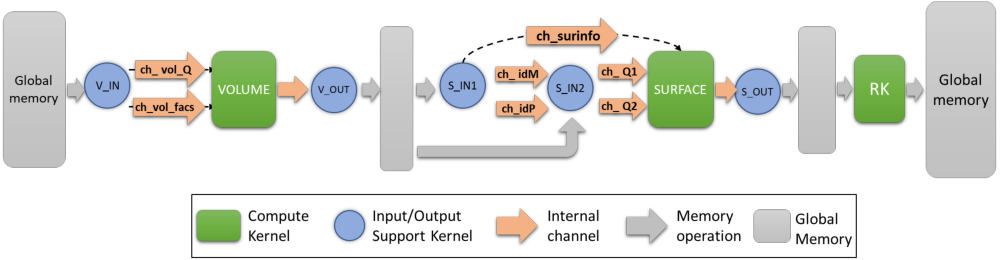
\includegraphics[width=1.0\textwidth]{images/nb_kernstruc}
    \caption{Block level structure for OpenCL™ kernels developed for single FPGA by \textcite{kenter_opencl-based_2018}}
    \label{fig:singlefpga_kernstruc}
\end{figure}

\TODO{Add details of the design}

\section{MIDG2 MPI FPGA implementation}
\label{sec:midg2_mpi}

The original MIDG2 implementation supports multi-node system with accelerators using
kernels for GPU. These kernels perform the shared data communication via \texttt{Host Application}
using MPI. Before the start of the thesis, as preparation phase, we extended the MIDG2 FPGA
implementation to work on a multi-node cluster with multiple FPGA accelerators to create MIDG2 MPI FPGA design.
The MIDG2 \ac{MPI} FPGA design uses the same code base as the original MIDG2 \ac{MPI} implementation
along with the modifications done to support OpenCL framework for FPGAs.
The mesh is divided into partitions using ParMETIS and the computation can be performed on different
compute nodes using FPGA accelerators. The OpenCL kernels from the MIDG2 FPGA design are used to replace
the original MIDG2 kernels for GPUs. An additional kernel which was used in the original MIDG2
implementation is included with necessary modification and used to read the shared data and store it in a coalesced
memory. A detailed information of the updated kernel structure is given in section \ref{sec:midge_mpi_struc}.
The updated \texttt{host application} then reads this data from the FPGA global memory and uses
\ac{MPI} to transfer it to other nodes to which the data is shared. Figure
\ref{fig:mpi_fpga} shows the system level architecture of this design for two nodes.
\begin{figure}[ht]%
    \centering
    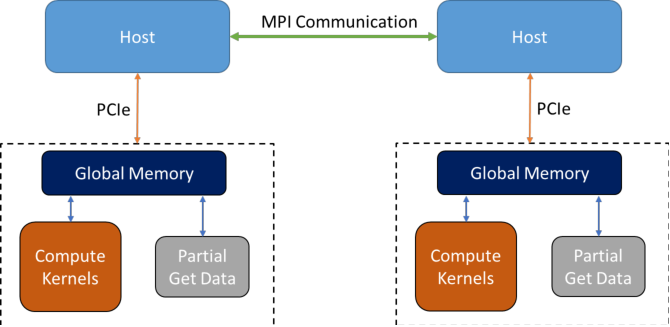
\includegraphics[width=0.8\textwidth]{images/mpi_fpga}
    \caption{System level architecture for MPI FPGA design communicating using MPI and PCIe}
    \label{fig:mpi_fpga}
\end{figure}

Using this design, multiple FPGAs can be used to speed up the computation for large meshes.
Though speedup can be achieved with this design, the communication which involves
movement of data through PCIe bus and the network interconnect between the nodes,
reduces the combined communication bandwidth a lot. This communication setup also
requires to have synchronization constructs between the FPGA kernels and the host
application to ensure data correctness which has overheads and contribute to the increase
of the overall execution time. This thesis uses this design as the base versions and replaces
the communication with point-to-point communication between FPGAs which allows
removing the complex communication and synchronization steps and speed up the
execution even further.

\subsection{OpenCL Kernel Structure of MIDG2 MPI FPGA Implementation}
\label{sec:midge_mpi_struc}

The MIDG2 FPGA implementation works for a single FPGA and utilizes special OpenCL FPGA
APIs and techniques to reduce the computation time for the electric and magnetic flux values
as explained in section \ref{sec:fpga_dg}. In a distributed MIDG2 application the shared
surfaces are identified after the mesh partition and a list of the shared nodes on the
surfaces is prepared which is used to share the data.
To exchange this shared data, MIDG2 FPGA kernels required a way to collect the shared
data in the FPGA global memory which the \texttt{host application} could then read and
exchange via MPI. To enable this, we added an additional \texttt{partial\_get\_kernel}
kernel to the design to gather the shared elements from
the main element buffer \texttt{g\_Q} into a smaller buffer partial data buffer \texttt{g\_partQ}.
The main benefit of using the additional kernel was to avoid the large memory transaction between the
host and the FPGA over PCIe to get the \texttt{g\_Q} and assemble the shared buffers in host.

The addition of the partial kernel was accompanied with re-shuffling of the elements in the \texttt{g\_Q}
buffer. The distributed design requires the mesh to be partitioned into smaller meshes allocated
to each rank. The elements of the partitioned mesh can either share a face with a neighboring
rank or within the rank. The elements which share faces with neighboring ranks form the shared
element group and the ones sharing faces within rank form the non-shared element group.
To separate the computation of the these shared element group and the non-shared element group
by reusing the same kernels required sorting of the elements into groups. This was done by
placing the shared elements in the start of the \texttt{g\_Q} buffer followed by the non-shared
elements as shown in figure \ref{fig:rearrange}. This allowed to use the same kernels with different
start and end element parameters to be invoked for processing the shared and non-shared elements separately.
\begin{figure}%
    \centering
    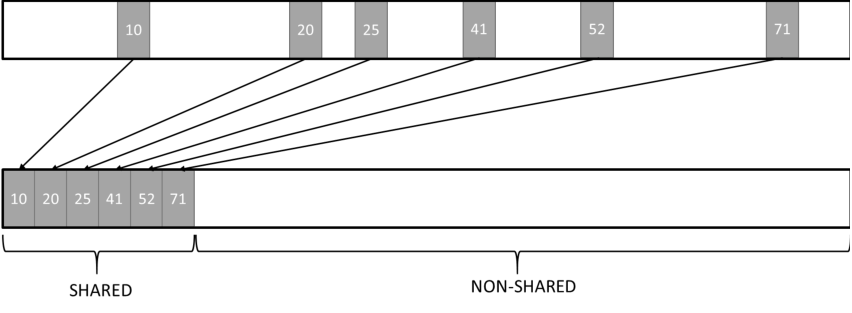
\includegraphics[width=0.6\textwidth]{images/rearrange}
    \caption{Rearrangement of \texttt{g\_Q} buffer elements by sorting and bringing the
    shared elements in the beginning of the buffer}
    \label{fig:rearrange}
\end{figure}

Prior to start of the thesis, we further optimized the original pipeline developed in MIDG2 FPGA
by introducing separate buffers \texttt{volrhsQ} and \texttt{surrhsQ} instead of the single
right hand side \texttt{rhsQ} buffer which was earlier accumulated in surface kernel.
This change allows the \texttt{VOLUME} and surface kernel to execute parallely and write data into
two separate buffers. The \texttt{RK} kernel reads both the buffers after \texttt{VOLUME} and surface kernel
are finished processing shared and non-shared data and accumulates the values using Runge-Kutta
constants to produce the field values for the timestep. The sequence of operations
showing the overlapped execution of the surface and \texttt{VOLUME} kernel is shown in figure \ref{fig:seq_singlefpga}.

\begin{figure}[ht]%
    \centering
    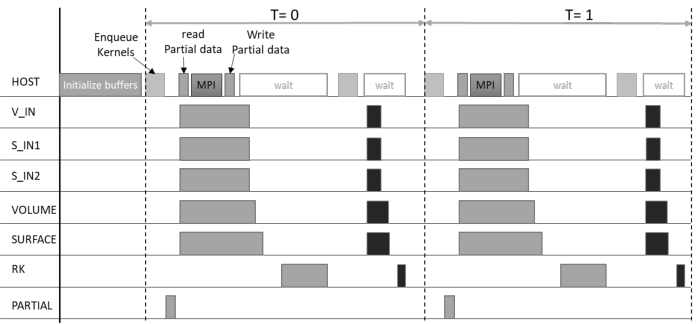
\includegraphics[width=0.8\textwidth]{seq_singlefpga}
    \caption{Sequence of MIDG2 MPI FPGA OpenCL kernels after including \texttt{volrhsQ} and \texttt{surrhsQ}
    showing them executing simultaneously}
    \label{fig:seq_singlefpga}
\end{figure}

Another improvement introduced before the thesis
to optimize the design was to use the concept of double buffers for the \texttt{g\_Q}.
The \texttt{g\_Q} buffer is duplicated into two buffers \texttt{g\_Q\_ping} and \texttt{g\_Q\_pong}
which use two aliases \texttt{g\_Q\_in} and \texttt{g\_Q\_out} in the kernel. The \texttt{g\_Q\_in}
serves as the buffer from which the kernels read the elements values for the current iteration whereas
\texttt{g\_Q\_out} serves as buffer in which the values
are updated. After each time step iteration the alias of the buffers is switched as shown
in pseudo code in \ref{code:buff_switch}, exchanging the functionality of the buffers for the next iteration.
\begin{CppCode}[caption=Buffer switching for double buffers in each iteration, frame=tlrb, label=code:buff_switch]
for (itr = 0; itr < MaxTimeStep; itr++)
{
    if (buffSwitch)
    {
        set_argument("g_Q_in", Q1_pong_mem);
        set_argument("g_Q_out", Q1_ping_mem);
    }
    else
    {
        set_argument("g_Q_in", Q1_ping_mem);
        set_argument("g_Q_out", Q1_pong_mem);
    }
    buffSwitch = !buffSwitch;
}
\end{CppCode}

This concept helps to improve the performance of the \texttt{RK} kernel
by removing read and write memory dependency on the same buffer and also allows executing
\texttt{RK} individually for shared and non-shared data as shown in figure \ref{fig:seq_singlefpga}.
In each time step, the \texttt{VOLUME} kernel and \texttt{SURFACE} kernel first execute to compute the right hand side values for the
non-shared elements while the shared data is exchanged. After computation is finished, \texttt{RK} kernel Once the shared data is available,
the right hand side values for the shared elements is computed. After the computation,
the \texttt{RK} kernels reads the field values from \texttt{g\_Q\_in} and \texttt{resQ} values
for the last time steps and computes the accumulated field values using
\texttt{volrhsQ} and \texttt{surrhsQ}. The computed values are then saved in \texttt{g\_Q\_out}.
As the read and write buffers are separated, the memory dependency on the same buffer is reduced,
reducing the latency to read and write to the memory. As explained, this structure also allows
to overlap the communication via MPI with the computation of the fields for the non-shared data
and reducing the effects of delayed communication. The kernel structure for base MPI MIDG2 FPGA
is shown in Figure \ref{fig:base_kernstruc}.
\begin{figure}[]%
    \centering
    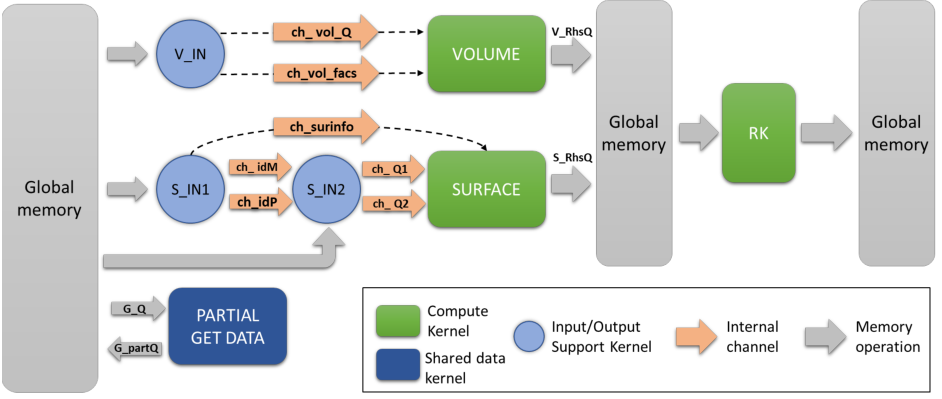
\includegraphics[width=1.0\textwidth]{images/base_kernstruc}
    \caption{Structure for MIDG2 MPI FPGA OpenC kernels showing the new partial get kernel used to gather
     the shared elements into a separate buffer \texttt{g\_partQ} for host to read. It also shows the introduction
     of \texttt{volrhsQ} and \texttt{surrhsQ} which allows the kernels to execute simultaneously as shown}
    \label{fig:base_kernstruc}
\end{figure}